% ─────────────────────────────────────────────────
%  ANNEXES
% ─────────────────────────────────────────────────
\appendix
\renewcommand{\chaptername}{Annexe}

% Affiche automatiquement une capture si le fichier a été ajouté ;
% conserve un emplacement explicite tant que l'image est absente.
\newcommand{\captureannexe}[4]{%
  \IfFileExists{#1}{%
    \includegraphics[width=#2\textwidth]{#1}%
  }{%
    \begin{emplacementcapture}{Capture à insérer : \texttt{#3}}%
      #4%
    \end{emplacementcapture}%
  }%
}

% ═════════════════════════════════════════════════
%  ANNEXE A – Interfaces complémentaires du parcours client SGI
% ═════════════════════════════════════════════════
\chapter{Interfaces complémentaires du parcours client SGI}
\markboth{Interfaces complémentaires SGI}{Interfaces complémentaires SGI}
\label{ann:interfaces-client-sgi}

Le chapitre~4 a présenté les résultats du module SGI du point de vue du
gestionnaire (tableau de bord, cotations, portefeuilles). La présente annexe
complète cette vue en illustrant le parcours tel qu'il est vécu par le
\textbf{client} : depuis la consultation de son portefeuille jusqu'à la
soumission d'un ordre d'investissement.

Les informations personnelles et financières affichées dans les interfaces de
cette annexe sont des données fictives de démonstration. De même, les données
de marché utilisées dans les vues SGI sont simulées, l'accès à un flux officiel
BRVM n'étant pas encore disponible dans l'environnement de validation.

Trois interfaces sont présentées :
\begin{itemize}
  \item la consultation du portefeuille client
        (figure~\ref{fig:ann_portefeuille_client}) ;
  \item la fiche détaillée d'un titre coté sur la BRVM
        (figure~\ref{fig:ann_detail_titre}) ;
  \item le formulaire de saisie d'un ordre d'achat ou de vente
        (figure~\ref{fig:ann_passage_ordre}).
\end{itemize}

\section{Consultation du portefeuille}

L'interface de consultation du portefeuille permet au client de visualiser la
composition et la valorisation de ses actifs avant toute décision
d'investissement. Elle affiche les positions détenues, leur cours actuel et
la performance associée.

\begin{figure}[H]
    \centering
    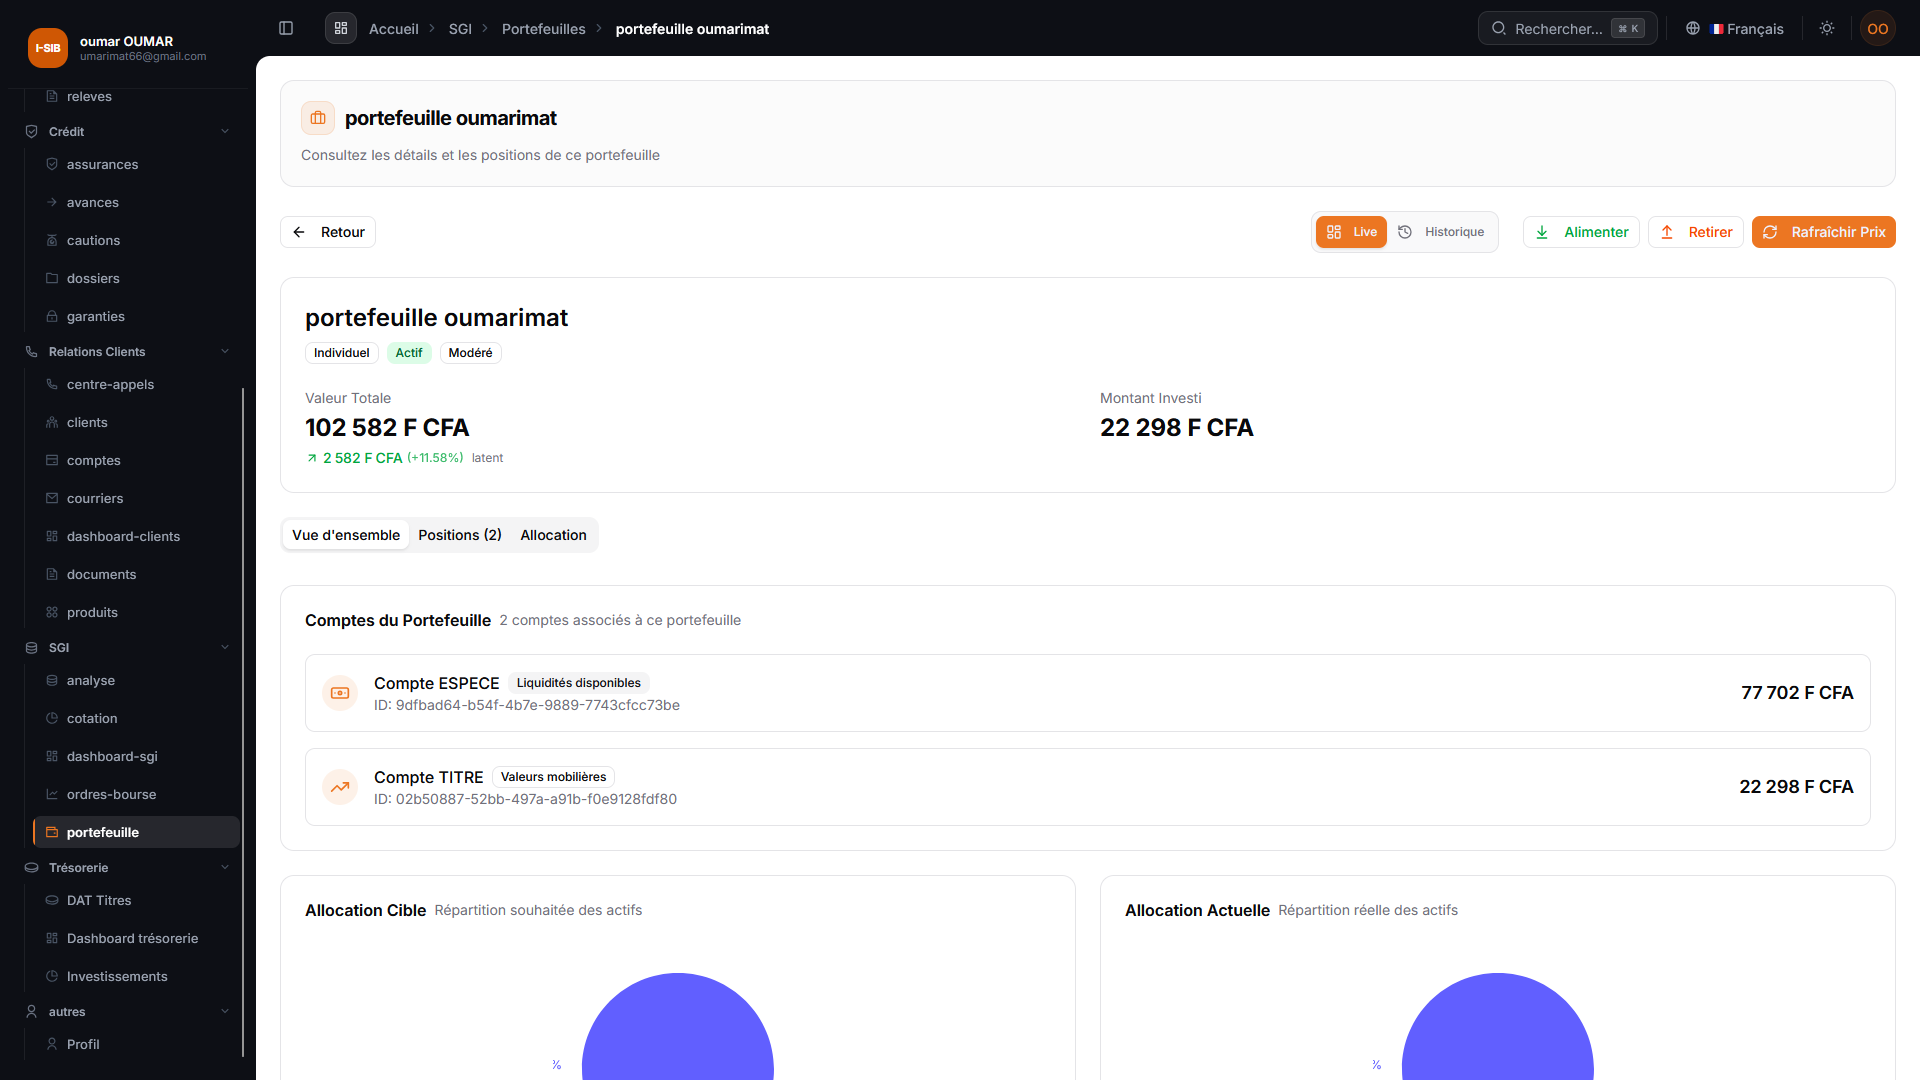
\includegraphics[width=0.86\textwidth]{images/annexes/annexe_a/annexe_a_portefeuille_client.png}
    \caption{Consultation du portefeuille côté client}
    \label{fig:ann_portefeuille_client}
\end{figure}

\section{Consultation d'un titre}

La fiche d'un titre présente les informations nécessaires à la prise de
décision : cours actuel, variation, volume échangé, historique de cotation
et caractéristiques de l'instrument. Cette vue précède la saisie d'un ordre.

\begin{figure}[H]
    \centering
    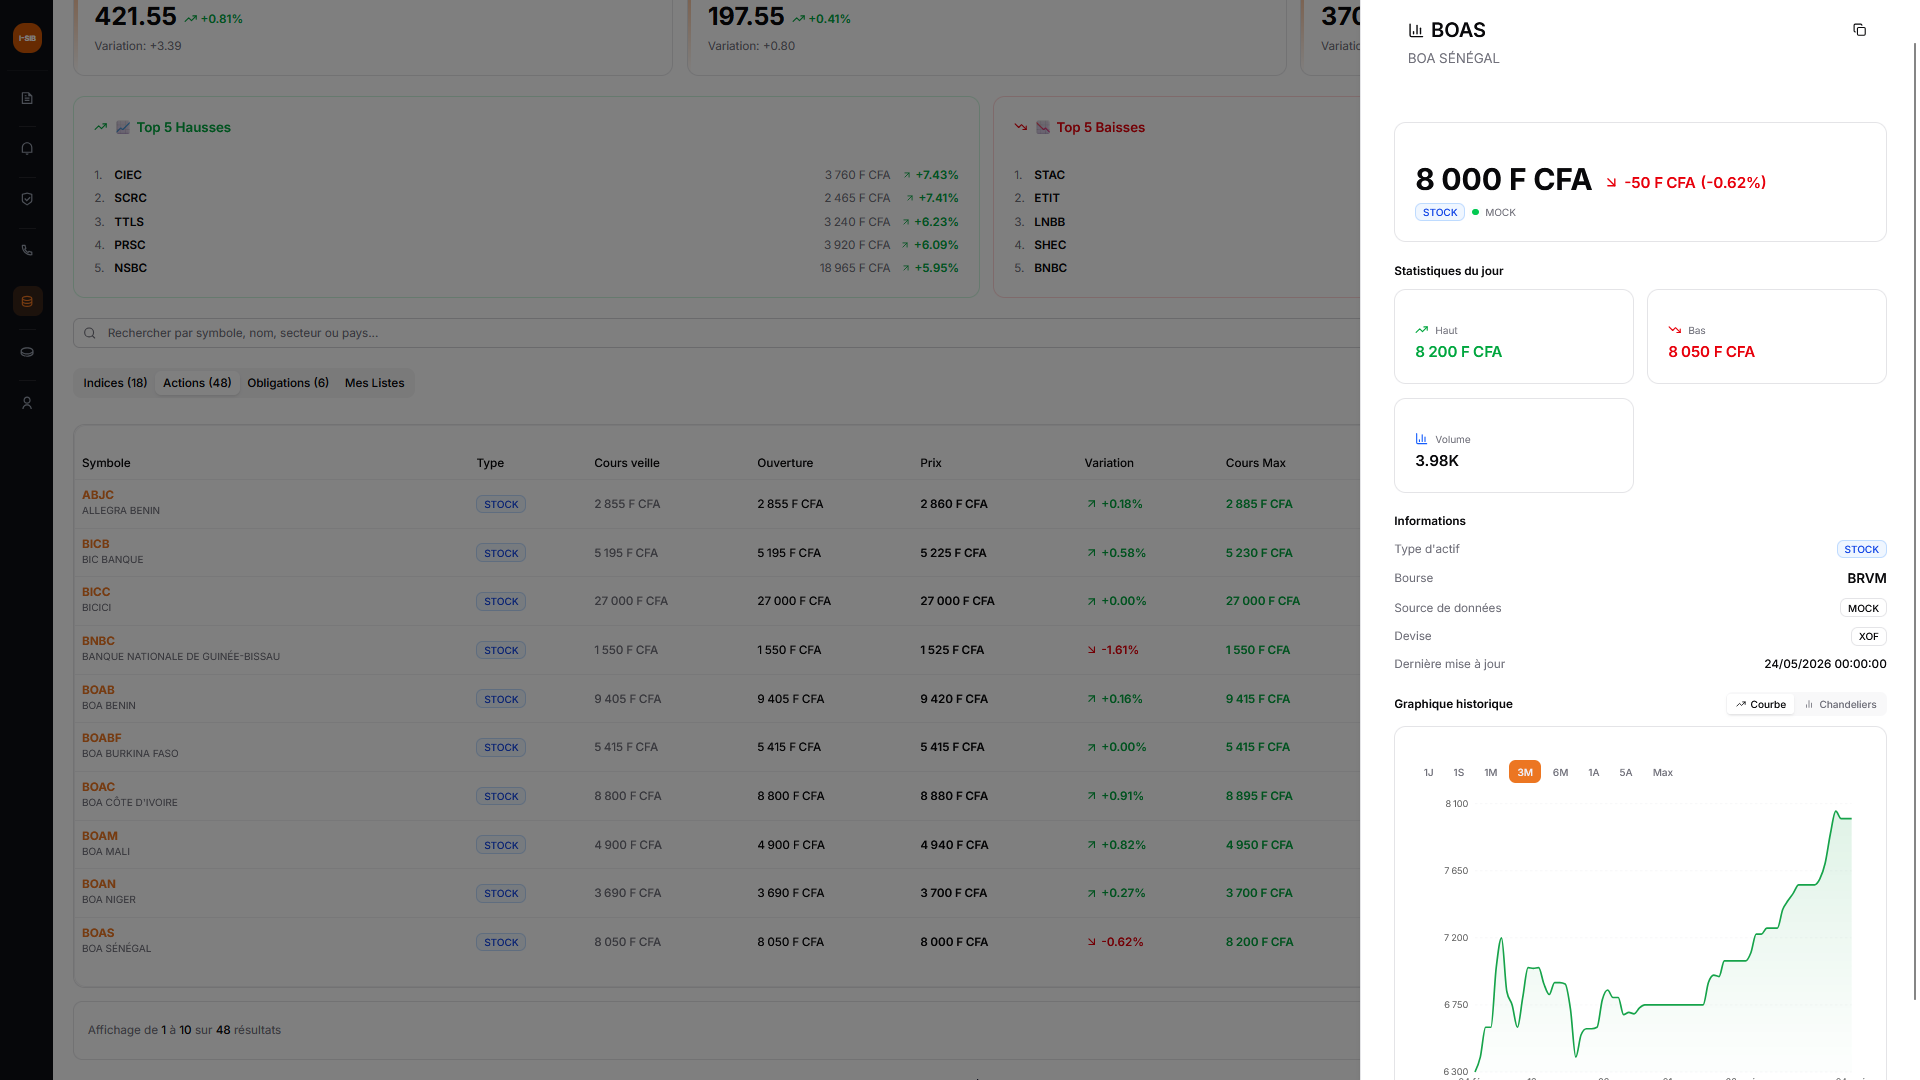
\includegraphics[width=0.86\textwidth]{images/annexes/annexe_a/annexe_a_detail_titre_client.png}
    \caption{Fiche d'un titre BRVM affichée avec des données simulées}
    \label{fig:ann_detail_titre}
\end{figure}

\section{Saisie d'un ordre}

Le formulaire de passage d'ordre permet au client de soumettre une intention
d'achat ou de vente sur un instrument coté. Une fois soumis, l'ordre suit le
workflow de traitement décrit au chapitre~2 : saisie, prise en charge par
l'équipe SGI, validation puis exécution.

\begin{figure}[H]
    \centering
    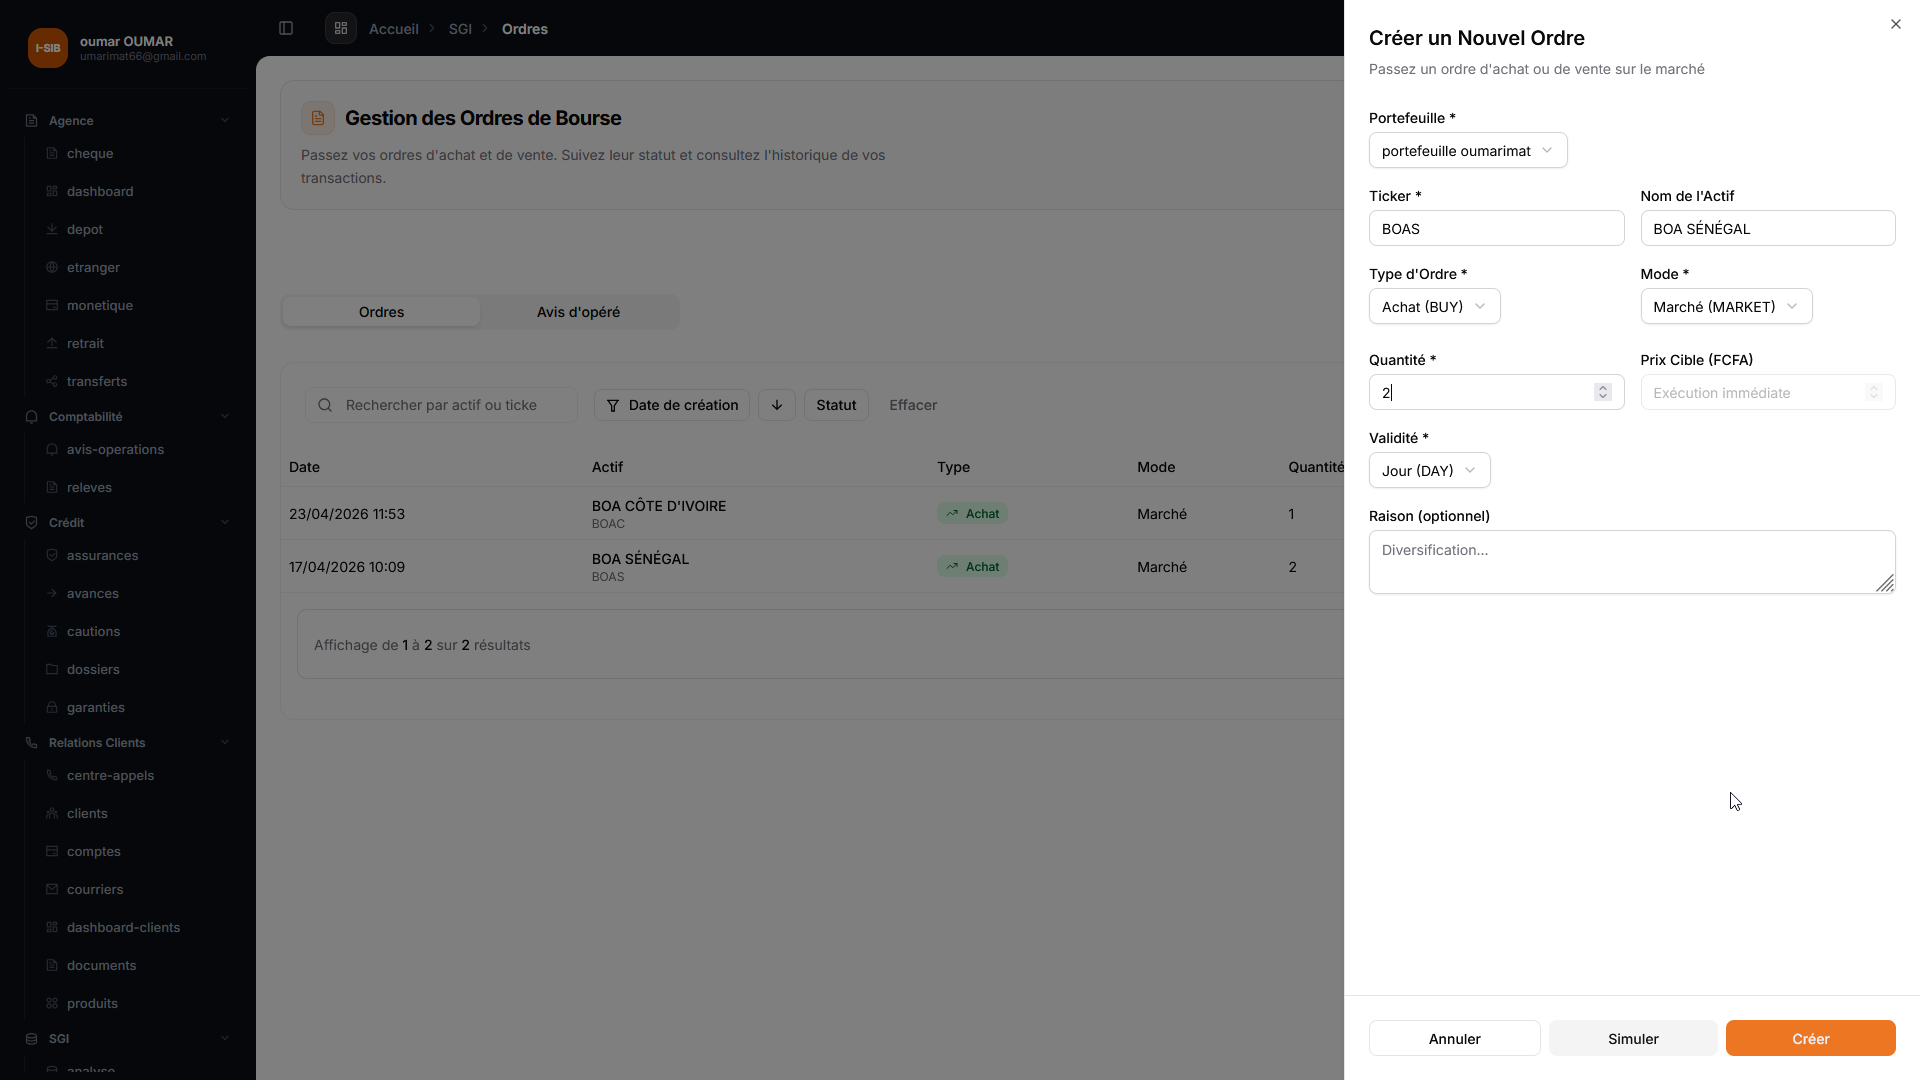
\includegraphics[width=0.86\textwidth]{images/annexes/annexe_a/annexe_a_passage_ordre_client.png}
    \caption{Formulaire de saisie d'un ordre d'investissement}
    \label{fig:ann_passage_ordre}
\end{figure}

% ═════════════════════════════════════════════════
%  ANNEXE B – Recette fonctionnelle de la gestion des prospects
% ═════════════════════════════════════════════════
\chapter{Recette fonctionnelle de la gestion des prospects}
\markboth{Recette fonctionnelle des prospects}{Recette fonctionnelle des prospects}
\label{ann:recette-fonctionnelle}

Cette annexe prolonge la conception détaillée volontairement centrée sur la
gestion des prospects aux chapitres~2 et~3. Elle documente, par des captures
de recette, le cheminement de deux scénarios représentatifs : l'enregistrement
d'un prospect avec calcul de son score, puis sa conversion en client. Les
captures attendues présentent l'action déclenchée par l'utilisateur et le
résultat produit par le système dans l'environnement de validation.
Les informations saisies et affichées dans ces captures sont des données
fictives utilisées exclusivement pour la recette fonctionnelle.

Deux scénarios sont documentés :
\begin{itemize}
  \item la création d'un prospect, depuis le formulaire de saisie jusqu'à
        l'affichage du prospect créé avec son score initial
        (figures~\ref{fig:recette_saisie_prospect} et~\ref{fig:recette_creation}) ;
  \item la conversion d'un prospect qualifié en client et l'observation du
        résultat de ce traitement
        (figures~\ref{fig:recette_conversion} et~\ref{fig:recette_conversion_preuve}).
\end{itemize}

Le tableau~\ref{tab:pieces_recette_annexe} récapitule les actions de recette,
les résultats vérifiables et les pièces justificatives prévues. La mention
\textit{Conforme} ne devra être portée qu'après insertion d'une capture
correspondant effectivement au résultat observé.

\begin{table}[H]
\centering
\caption{Vérifications de recette de la gestion des prospects}
\label{tab:pieces_recette_annexe}
\footnotesize
\renewcommand{\arraystretch}{1.18}
\begin{tabularx}{\textwidth}{|p{2.65cm}|p{3.25cm}|X|p{2.55cm}|}
\hline
\textbf{Scénario} & \textbf{Action exécutée} &
\textbf{Résultat attendu / observé} & \textbf{Preuve / statut} \\ \hline
Création d'un prospect &
Soumettre un formulaire de prospect renseigné. &
Attendu : prospect enregistré avec score initial. Observé : à confirmer par
la recette. &
Figures~\ref{fig:recette_saisie_prospect}--\ref{fig:recette_creation} /
à documenter. \\ \hline
Conversion en client &
Déclencher la conversion d'un prospect qualifié. &
Attendu : statut converti et client créé. Observé : à confirmer par la recette. &
Figures~\ref{fig:recette_conversion}--\ref{fig:recette_conversion_preuve} /
à documenter. \\ \hline
\end{tabularx}
\end{table}

\section{Création d'un prospect}

La création d'un prospect commence par la saisie des informations commerciales
nécessaires depuis l'interface du chargé de clientèle. Après validation, le
service CRM enregistre le prospect et sollicite le service de scoring afin
d'associer un score initial au nouveau contact. Les deux figures suivantes
permettront de rapprocher l'entrée utilisateur du résultat obtenu.

\begin{figure}[H]
\centering
\captureannexe{images/annexes/annexe_b/annexe_b_formulaire_creation_prospect.png}{0.88}
{annexe\_b\_formulaire\_creation\_prospect.png}
{Capture attendue du formulaire renseigné pour enregistrer un nouveau prospect.}
\caption{Saisie d'un nouveau prospect par le chargé de clientèle}
\label{fig:recette_saisie_prospect}
\end{figure}

\begin{figure}[H]
\centering
\captureannexe{images/annexes/annexe_b/annexe_b_prospect_cree_score.png}{0.88}
{annexe\_b\_prospect\_cree\_score.png}
{Capture attendue du prospect créé dans le pipeline avec son score initial.}
\caption{Prospect enregistré avec score initial calculé}
\label{fig:recette_creation}
\end{figure}

\section{Conversion d'un prospect en client}

La conversion est déclenchée sur un prospect qualifié ; il ne s'agit pas d'une
simple modification manuelle de statut. Le workflow décrit au chapitre~3
sollicite la segmentation, crée le client, initialise les traitements associés,
met à jour le prospect en état converti et envoie le courriel de bienvenue. Les
figures ci-dessous accueilleront la preuve du résultat principal, puis une
preuve complémentaire issue du client créé, de son compte ou du message généré.

\begin{figure}[H]
\centering
\captureannexe{images/annexes/annexe_b/annexe_b_prospect_converti.png}{0.88}
{annexe\_b\_prospect\_converti.png}
{Capture attendue du prospect après déclenchement de la conversion, avec statut converti.}
\caption{Prospect converti en client à l'issue du workflow}
\label{fig:recette_conversion}
\end{figure}

\begin{figure}[H]
\centering
\captureannexe{images/annexes/annexe_b/annexe_b_preuve_client_cree.png}{0.88}
{annexe\_b\_preuve\_client\_cree.png}
{Capture complémentaire attendue du client créé, de son compte ou du courriel de bienvenue.}
\caption{Preuve complémentaire générée par la conversion du prospect}
\label{fig:recette_conversion_preuve}
\end{figure}

% ═════════════════════════════════════════════════
%  ANNEXE C – Module Manager et audit des opérations
% ═════════════════════════════════════════════════
\chapter{Module Manager et audit des opérations}
\markboth{Module Manager et audit}{Module Manager et audit}
\label{ann:administration-acces}

Dans un contexte bancaire, la maîtrise des habilitations et la traçabilité
des opérations participent à la sécurisation des parcours métier. La
plateforme I-SIB intègre un \textbf{module Manager} destiné à la gestion des
modules, des fonctionnalités et des rôles autorisés pour chaque
fonctionnalité. Elle propose également, dans le back-office
d'administration, une section \textbf{Audit} permettant de consulter les
requêtes et actions enregistrées.

Cette annexe présente la traduction fonctionnelle de ces mécanismes dans
l'environnement de validation. Les captures attestent de l'existence des
interfaces Manager et Audit ; elles ne remplacent pas une campagne
exhaustive de tests d'autorisation ni un audit de sécurité avant production.

\begin{table}[H]
\centering
\caption{Éléments de preuve relatifs aux accès et à l'audit}
\label{tab:preuves_acces_audit}
\footnotesize
\renewcommand{\arraystretch}{1.18}
\begin{tabularx}{\textwidth}{|p{3.35cm}|X|p{3.15cm}|p{2.1cm}|}
\hline
\textbf{Vérification} & \textbf{Résultat attendu} &
\textbf{Preuve} & \textbf{Statut} \\ \hline
Gestion du référentiel d'accès &
Modules et fonctionnalités administrables depuis le module Manager. &
Figure~\ref{fig:ann_modules_permissions} & À documenter \\ \hline
Paramétrage par rôle &
Rôles autorisés configurés pour une fonctionnalité métier. &
Figure~\ref{fig:ann_roles_fonctionnalite} & À documenter \\ \hline
Consultation de l'audit &
Requêtes et opérations consultables depuis l'administration. &
Figure~\ref{fig:ann_journal_audit} & À documenter \\ \hline
\end{tabularx}
\end{table}

\section{Module Manager : gestion des accès}

Le module Manager permet d'administrer le référentiel fonctionnel de la
plateforme : modules, fonctionnalités associées et rôles habilités à les
utiliser. Une première capture présente l'interface générale de gestion ; la
seconde illustre le paramétrage des rôles autorisés pour une fonctionnalité
du périmètre étudié.

\begin{figure}[H]
\centering
\captureannexe{images/annexes/annexe_c/annexe_c_modules_permissions.png}{0.88}
{annexe\_c\_modules\_permissions.png}
{Capture attendue du module Manager présentant les modules et fonctionnalités administrables.}
\caption{Gestion des modules et fonctionnalités depuis le module Manager}
\label{fig:ann_modules_permissions}
\end{figure}

\begin{figure}[H]
\centering
\captureannexe{images/annexes/annexe_c/annexe_c_roles_fonctionnalite.png}{0.88}
{annexe\_c\_roles\_fonctionnalite.png}
{Capture attendue des rôles configurés pour une fonctionnalité, par exemple la gestion des prospects.}
\caption{Paramétrage des rôles autorisés pour une fonctionnalité}
\label{fig:ann_roles_fonctionnalite}
\end{figure}

\section{Back-office d'administration : audit des requêtes}

La section Audit du back-office d'administration permet de consulter les
requêtes et actions enregistrées dans la plateforme. Cette vue contribue au
suivi des opérations sensibles et à l'analyse d'incidents éventuels.

\begin{figure}[H]
\centering
\captureannexe{images/annexes/annexe_c/annexe_c_journal_audit.png}{0.88}
{annexe\_c\_journal\_audit.png}
{Capture attendue de la section Audit affichant les requêtes et opérations enregistrées.}
\caption{Consultation des requêtes tracées dans la section Audit}
\label{fig:ann_journal_audit}
\end{figure}

% ═════════════════════════════════════════════════
%  ANNEXE D – Validation du déploiement sur VPS AlmaLinux
% ═════════════════════════════════════════════════
\chapter{Validation du déploiement sur VPS AlmaLinux}
\markboth{Validation du déploiement}{Validation du déploiement}
\label{ann:validation-deploiement}

Cette dernière annexe rassemble les preuves visuelles de l'environnement de
validation présenté au chapitre~3. Une fois les captures insérées, elle
documentera l'état des composants I-SIB déployés sur le VPS AlmaLinux utilisé
pour la recette.

Trois éléments sont documentés :
\begin{itemize}
  \item l'état des conteneurs Docker via l'interface Portainer
        (figure~\ref{fig:ann_portainer}) ;
  \item l'enregistrement des microservices dans le registre Eureka
        (figure~\ref{fig:ann_eureka}) ;
  \item l'historique de redéploiement attestant du processus itératif
        de mise à jour (figure~\ref{fig:ann_redeploiement}).
\end{itemize}

Le tableau~\ref{tab:preuves_deploiement} présente les contrôles à appuyer par
les captures du serveur. Les statuts seront confirmés lorsque les pièces issues
du VPS auront été ajoutées au mémoire.

\begin{table}[H]
\centering
\caption{Preuves attendues du déploiement de validation}
\label{tab:preuves_deploiement}
\footnotesize
\renewcommand{\arraystretch}{1.18}
\begin{tabularx}{\textwidth}{|p{3.2cm}|X|p{3.25cm}|p{2.15cm}|}
\hline
\textbf{Vérification} & \textbf{Résultat attendu} &
\textbf{Preuve} & \textbf{Statut} \\ \hline
Conteneurs actifs &
Services I-SIB démarrés sur le VPS AlmaLinux. &
Figure~\ref{fig:ann_portainer} & À documenter \\ \hline
Découverte des services &
Microservices enregistrés et accessibles via l'infrastructure applicative. &
Figure~\ref{fig:ann_eureka} & À documenter \\ \hline
Redéploiement &
Historique montrant une mise à jour progressive des services. &
Figure~\ref{fig:ann_redeploiement} & À documenter \\ \hline
\end{tabularx}
\end{table}

\section{Services conteneurisés}

La capture Portainer permettra de vérifier l'état des conteneurs Docker des
quatre ensembles (infra, core, module, office) sur le serveur de validation.

\begin{figure}[H]
\centering
\captureannexe{images/annexes/annexe_d/annexe_d_portainer_conteneurs.png}{0.88}
{annexe\_d\_portainer\_conteneurs.png}
{Vue Portainer des conteneurs I-SIB actifs sur le VPS AlmaLinux.}
\caption{Conteneurs Docker actifs sur le VPS AlmaLinux}
\label{fig:ann_portainer}
\end{figure}

\section{Enregistrement des services}

Le tableau Eureka permettra de documenter les microservices enregistrés auprès
du registre de services et rendus disponibles à la passerelle API.

\begin{figure}[H]
\centering
\captureannexe{images/annexes/annexe_d/annexe_d_eureka_services.png}{0.88}
{annexe\_d\_eureka\_services.png}
{Tableau Eureka montrant les services applicatifs enregistrés et disponibles.}
\caption{Services enregistrés dans le registre Eureka}
\label{fig:ann_eureka}
\end{figure}

\section{Redéploiement progressif}

L'historique de redéploiement documentera le processus itératif de mise à jour
des services sur le serveur de validation, en cohérence avec la démarche
incrémentale adoptée pour le projet.

\begin{figure}[H]
\centering
\captureannexe{images/annexes/annexe_d/annexe_d_pipeline_redeploiement.png}{0.88}
{annexe\_d\_pipeline\_redeploiement.png}
{Capture attendue de l'historique de redéploiement sur le VPS de validation.}
\caption{Historique de redéploiement sur le serveur de validation}
\label{fig:ann_redeploiement}
\end{figure}
